\documentclass[11pt, letterpaper, oneside]{article}


%\usepackage{microtype}
%\usepackage[utf8]{inputenc}
%\usepackage[T1]{fontenc}
%\usepackage{titlesec}
%\usepackage{graphicx}
%\usepackage{enumitem}
%\usepackage{amsthm}
%%\setlist{nolistsep}
%\usepackage{tikz}
%\graphicspath{{images/}}
%
%\usepackage[utf8]{inputenc}
%\usepackage{amsmath}
%\usepackage{amsfonts}
%\usepackage{amssymb}
%\usepackage[left=2cm,right=2cm,top=2cm,bottom=2cm]{geometry}
%%\usepackage{color}
%\usepackage[usenames,dvipsnames]{xcolor}
%\usepackage{sectsty}
%\usepackage{framed}
%%\usepackage{tikz}
%
%% Font Settings
%\usepackage{avant}
%\usepackage{fourier} 
%\usepackage{charter}
%
%\theoremstyle{definition}
%\newtheorem{definition}{Definition}[section]
%\newtheorem{example}{Ex.}[section]
%\newtheorem{theorem}{Theorem}[section]
%

\usepackage{graphicx}
\graphicspath{{images/}} %image directory

\usepackage{amsmath}
\usepackage{amsfonts}
\usepackage{amssymb}
\usepackage{graphicx}
\usepackage{url}
\usepackage[top=25mm, bottom=25mm, left=30mm, right=25mm]{geometry}
\setlength{\parindent}{0cm} % first para - no indent
\usepackage{titlesec}
\usepackage{setspace}
\usepackage[nottoc]{tocbibind}
\usepackage{listings}
%\usepackage[table]{xcolor}
\usepackage{multirow}
\usepackage{pdflscape}
\usepackage{color}
\usepackage[usenames,dvipsnames]{xcolor}
\usepackage{fancyhdr}
\newtheorem{mydef}{Example}
\titlespacing*{\chapter}{0pt}{0pt}{20pt}
\usepackage{microtype}
\usepackage[toc,page]{appendix}

%\setlist{nolistsep}

% Font settings
\usepackage{avant}
\usepackage{fourier} 
\usepackage{charter}


% Header settings
%\titleformat{\chapter}{\Large\bfseries}{Chapter \thechapter }{14pt}{\Large}
%\titleformat{\chapter}{\Large\bfseries}{\thechapter }{14pt}{\Large}
\titleformat{\section}{\large\bfseries}{{\color{MidnightBlue}\thesection }}{13pt}{\color{MidnightBlue}\large}
\titleformat{\subsection}{\normalsize\bfseries}{ \color{NavyBlue}\thesubsection }{12pt}{\color{NavyBlue}\normalsize}
\titleformat{\paragraph}{\normalsize\bfseries}{ \thesection }{12pt}{\large}

% Itemize - remove exrea linespace
\newlength{\wideitemsep}
\setlength{\wideitemsep}{.5\itemsep}
\addtolength{\wideitemsep}{-7pt}
\let\olditem\item
\renewcommand{\item}{\setlength{\itemsep}{\wideitemsep}\olditem}

% Header and footer
\fancypagestyle{plain}{
\fancyhf{}
\renewcommand{\headrulewidth}{0pt}
\renewcommand{\footrulewidth}{0pt}
\fancyfoot[LE,RO]{\scriptsize{ \thepage} }
%\fancyfoot[RE,LO]{\small ODROID XU4 - Documentation}
%\fancyhead[RO,LE]{\scriptsize{FDCL Document}}
}

\definecolor{maroon}{RGB}{173,34,49}
\definecolor{shadecolor}{RGB}{233,244,255}
\definecolor{exframecolor}{RGB}{255,255,255}
\definecolor{exshadecolor}{RGB}{250,252,252}    
    

\newenvironment{exframe}{
\def\FrameCommand{\fboxrule=\FrameRule\fboxsep=\FrameSep \fcolorbox{exframecolor}{exshadecolor}}
\MakeFramed {\FrameRestore}}
{\endMakeFramed}

% For hyperlinks
\usepackage{hyperref}
\hypersetup{
    colorlinks,
    linkcolor={black!80!black},
    citecolor={blue!50!black},
    urlcolor={blue!80!black}
}

\usepackage{cleveref}  % automatic reference formatting (load AFTER hyperref)
\pagestyle{plain}


\title{Sumo Robot - Report}
\author{Kanishke Gamagedara \\ Kalpesh Patil}

\begin{document}
\thispagestyle{empty}

\begin{center}

%\begin{figure}[h!]
%\begin{center}
%\includegraphics[scale=1]{uni_crest.png}
%\end{center}
%\end{figure}

\vspace*{.5cm}

\title{ \bfseries Sumo Robot \\ Report}
\author{Kalpesh Patil \\ Kanishke Gamagedara\\ {\normalsize kanishkegb@gwu.edu}\\{\normalsize Fall 2016}}

\vspace{10 mm}
 {\bf \color{MidnightBlue} {\Huge Sumo Robot } \vspace{4mm} \hline  \vspace{4mm} {\Huge Report}}\\

\vspace*{6cm}

{\large This is the project report for the robot ``Interpreter'' made for the class MAE 6194 }

\vspace*{5cm}

{\large Kalpesh Patil \\ {\normalsize kalpeshpatil33@gwu.edu }\\ \vspace*{5mm} Kanishke Gamagedara}\\ 
{\normalsize kanishkegb@gwu.edu}\\\vspace*{5mm}{\large Spring 2017}

\vspace*{3cm}

{\LARGE 
The George Washington University}

\end{center}
\newpage



\tableofcontents


% =================================================================================
\newpage
\section{Summary}

\begin{figure}[bth]
	\begin{center}
		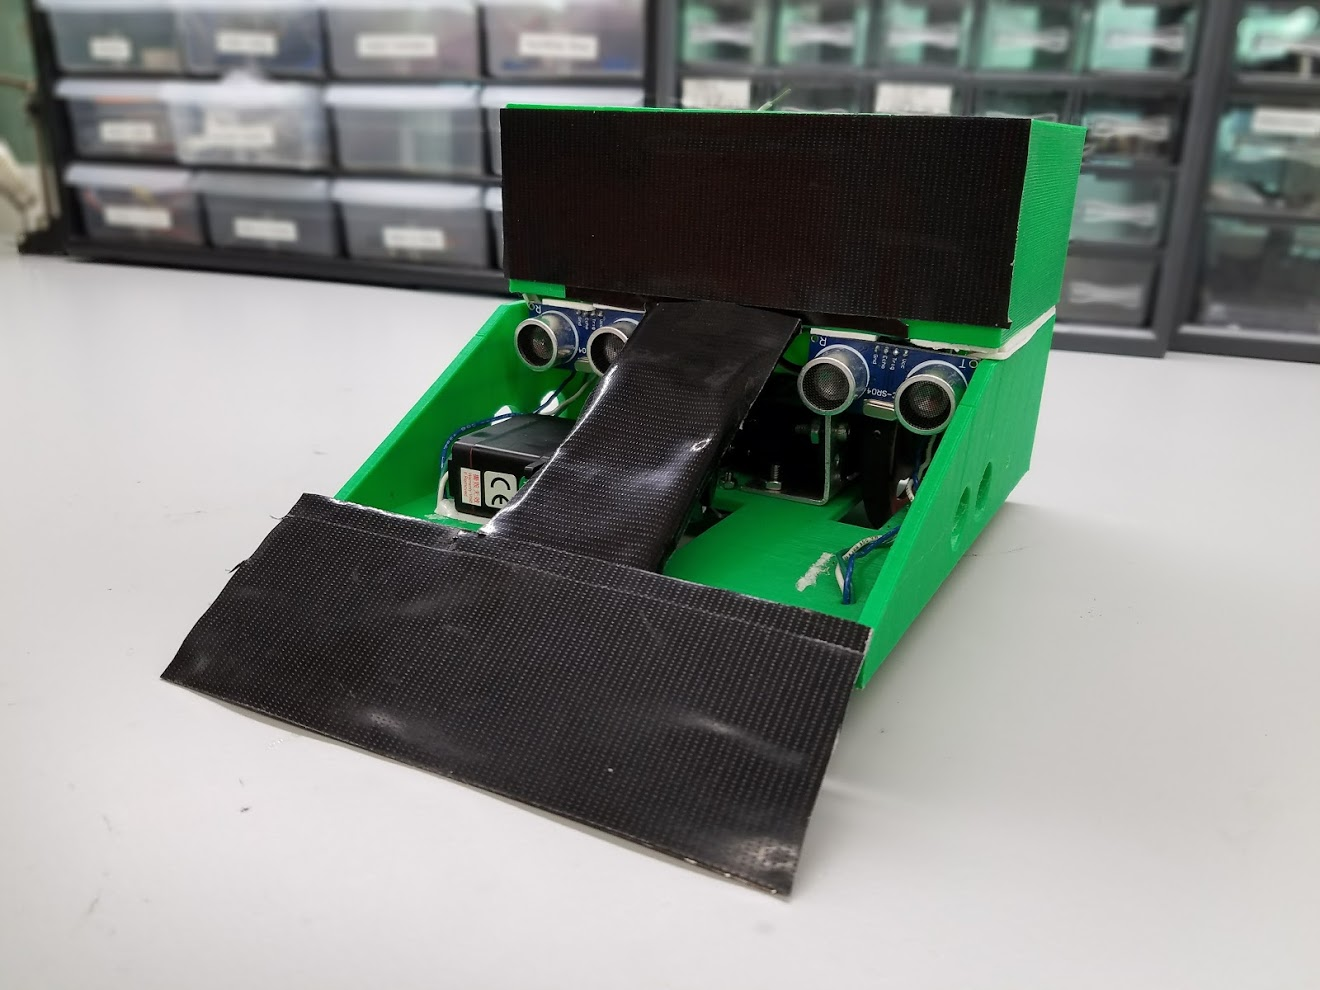
\includegraphics[scale = 0.2]{front.jpg}
		\caption{Interpreter}
		\label{fig:front}
	\end{center}
\end{figure}

We made the ``Interpreter'' for the Sumo Robot Competition, which was held as a part of the course MAE 6194. This robot has an LCD serial monitor, which is operated through XBee, which displays ( or interprets ) everything it does. This lead to the name Interpreter.  The basic functions and features of the robot are listed below.
\begin{itemize}
	\item Finds the opponent using sonar sensors
	\item Detects the line using QTI sensors
	\item If and opponent is detected, accelerates towards it
	\item If the opponent is close enough, raise the flipping shield
	\item Send every task the robot is performing through XBee
	\item Another Arduino board reads the transmitted data via an XBee, and prints to an LCD display
\end{itemize}

This report is organized as follows. First, we will discuss the details on the body structure and the sensors. Then we will be explaining how the attacking mechanism works. Next section is on details of the LCD serial monitor system which is used to continuously monitor and debug the robot. Then we will provide an overview of the overall algorithm which is used to control the robot. Finally the issues we faced and the proposed future developments. The codes are attached in the appendix.


% =================================================================================
\newpage
\section{Physical Structure}

\begin{figure}[bth]
	\begin{center}
		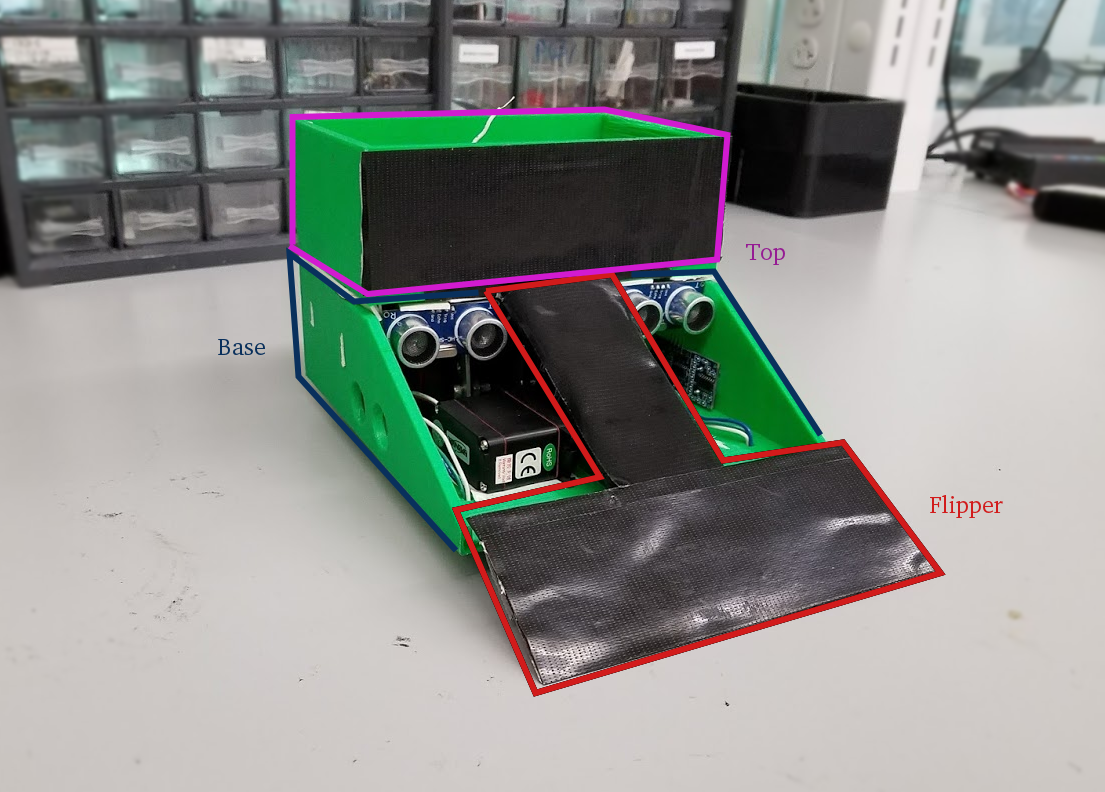
\includegraphics[scale = 0.3]{detailed_structure.png}
		\caption{Structure}
		\label{fig:detailed_structure}
	\end{center}
\end{figure}

In this section, we discuss about the body structure of the robot and the sensors. The robots structure mainly has three parts. 
\begin{enumerate}
	\item Base
	\item Top
	\item Flipper
\end{enumerate}


Base holds all the motors, back and side sonar sensors, and the QTI sensors at the bottom. On top of the Base, we have placed the Top which securely holds the Arduino board, batteries, Xbee unit, and the two front sonar sensors. Flipper is hinged to the front bottom edge of the Top and a servo motor with an arm is placed on the base, directly under the flipper, to activate the attacking mechanism.



% =================================================================================
\newpage
\section{Sensors and Components}
A physical structure of a robot is nothing without sensing or actuation devices. In this section, we describe the sensors and components we used on our robot. \\

\subsection{Line Detection}
The most important objective of a Sumo Robot is to detect the boundary line of the ring. For this, we used QTI sensors by Parallax\footnote{\url{https://www.parallax.com/product/555-27401}}, where QTI stands for Q - charge, T - transfer and, I - infrared. We used three QTI sensors, one in the center and two in the front left and front right.
\begin{figure}[bth]
	\begin{center}
		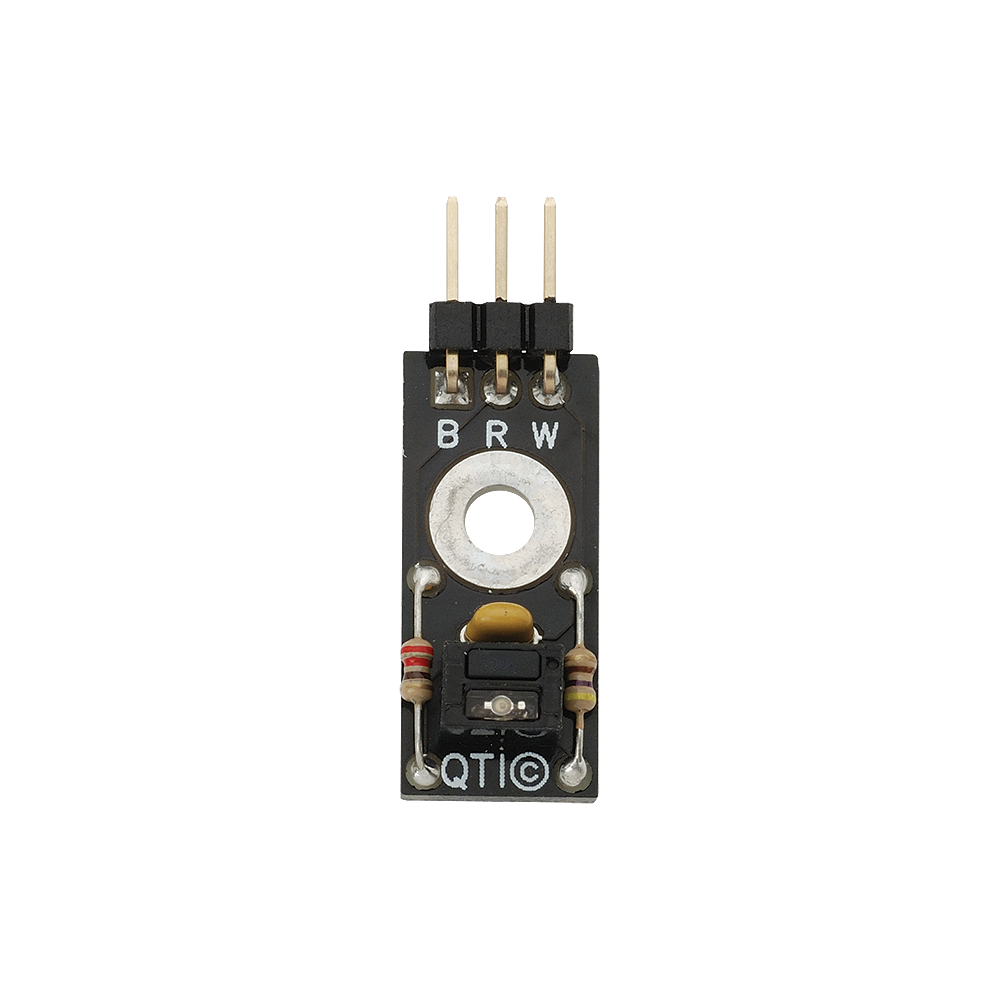
\includegraphics[scale = 0.15]{qti.png}
		\caption{QTI Sensor}
		\label{fig:qti}
	\end{center}
\end{figure}

Referring \cref{fig:qti}, pin W is supplied with 5 V and pin B is connected to the ground. Pin R is the sensor pin. As name implies, the sensor need to be charged. This is done by setting the sensor pin to HIGH during the initialization. In the case of middle QTI sensor, we need to shutdown the robot as soon as it detects the white line. For this, we used interrupts. Example code can be found below.

\begin{verbatim}
void setup() {
    pinMode(MIDDLE_pinQTIsensor, INPUT);  // set sensor pin as an input
    digitalWrite(MIDDLE_pinQTIsensor, HIGH);  // charging phase of the QTI
	
    attachInterrupt(digitalPinToInterrupt(MIDDLE_pinQTIsensor), MIDDLE_whiteLineISR, LOW);
    // attach the interrupt 
 }
 
void MIDDLE_whiteLineISR() {
    goStop();  // stop the robot as soon as middle QTI detects a line
}
\end{verbatim}


\subsection{Sonar Sensors}
The next objective of the robot is to identify the opponent robot. We used five HC-SR04 sonar sensors\footnote{\url{https://goo.gl/ZwPIIL}}. Two sensors were used in the front, and other three were used on left, right and back. The sensor sends a sonar signal and receives it back. The time difference between sending and receiving is used to calculate the distance of and obstacle. The sensor has a range of 2 - 500 cm for obstacle detection.
\begin{figure}[bth]
	\begin{center}
		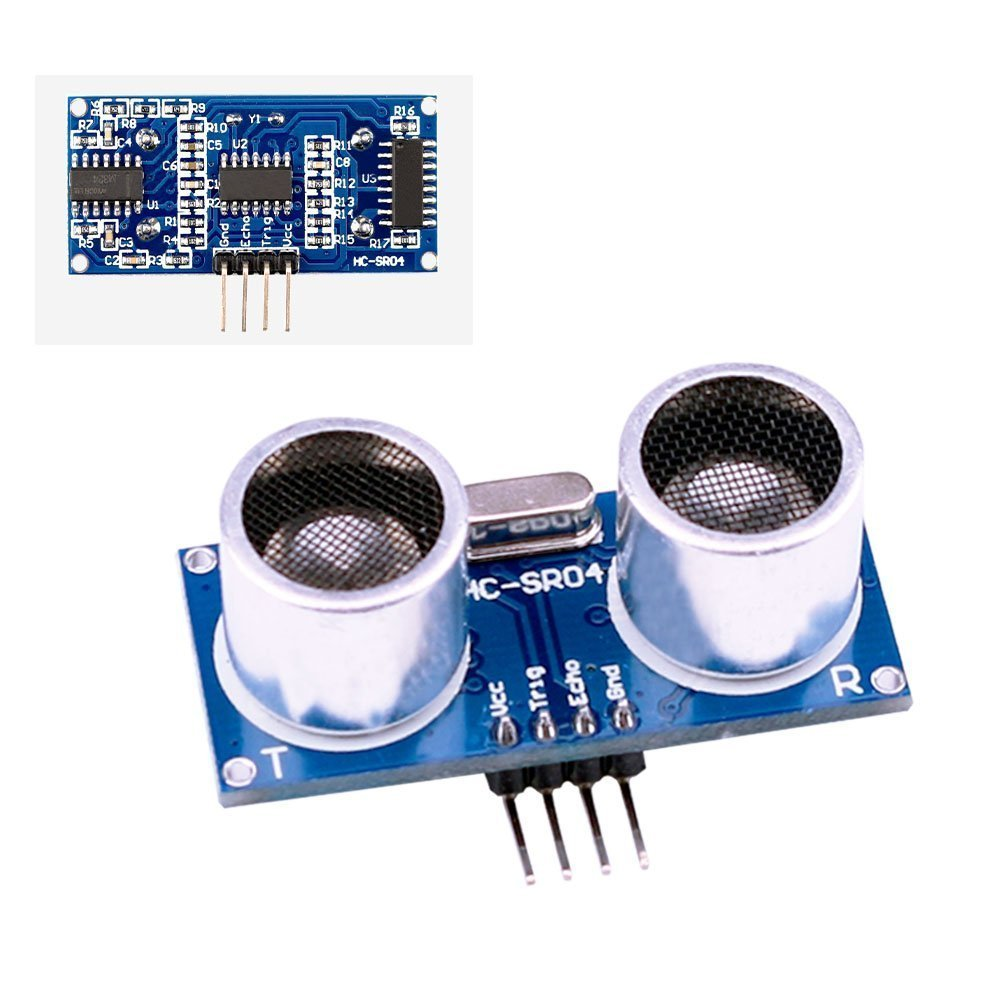
\includegraphics[scale = 0.15]{sonar.jpg}
		\caption{HC-SR04}
		\label{fig:sonar}
	\end{center}
\end{figure}

This sensor has four pins: power, ground, trigger, and echo. Power in is supplied with 5 V. We need to write the pulse to the trigger pin and then read the echo. For this we use built-in Arduino function ``pulseIn''\footnote{\url{https://www.arduino.cc/en/Reference/pulseIn}}. This function returns the time the length of the pulse in microseconds. Since we know that the speed of sound is $340 \; m/s = 0.034 \; cm / \mu s$, we can calculate the distance to the obstacle.

\begin{verbatim}
int FRONT_distance = 0  // initialize the distance to an obstacle facing front 
                        // sensor as a global variable

void FRONT_HC() {
    // writes the pulse
    digitalWrite(FRONT_trigPin, LOW);
    digitalWrite(FRONT_trigPin, HIGH);
    delay(100);                      
    digitalWrite(FRONT_trigPin, LOW);
    
    FRONT_duration = pulseIn(FRONT_echoPin, HIGH);  // read the echo
    FRONT_distance = (FRONT_duration / 2) * 0.034;  // calculate the distance
}

void loop {
    FRONT_HC();  // call the front sonar function
}
\end{verbatim}


\subsection{Motors}
Motors are the actuators of our robot. We used three motors: two for the motion of the robot and one for the attacking mechanism. For the wheel motors, we use Parallax continuous rotation servo motors\footnote{\url{https://www.parallax.com/product/900-00008}}. Each of the motors has a power pin ( 5 V ), ground pin, and a servo pin. In this section we mainly focus on wheel motors. The motor we used for the attacking mechanism is described in \cref{sec:attacking}.

\begin{figure}[bth]
	\begin{center}
		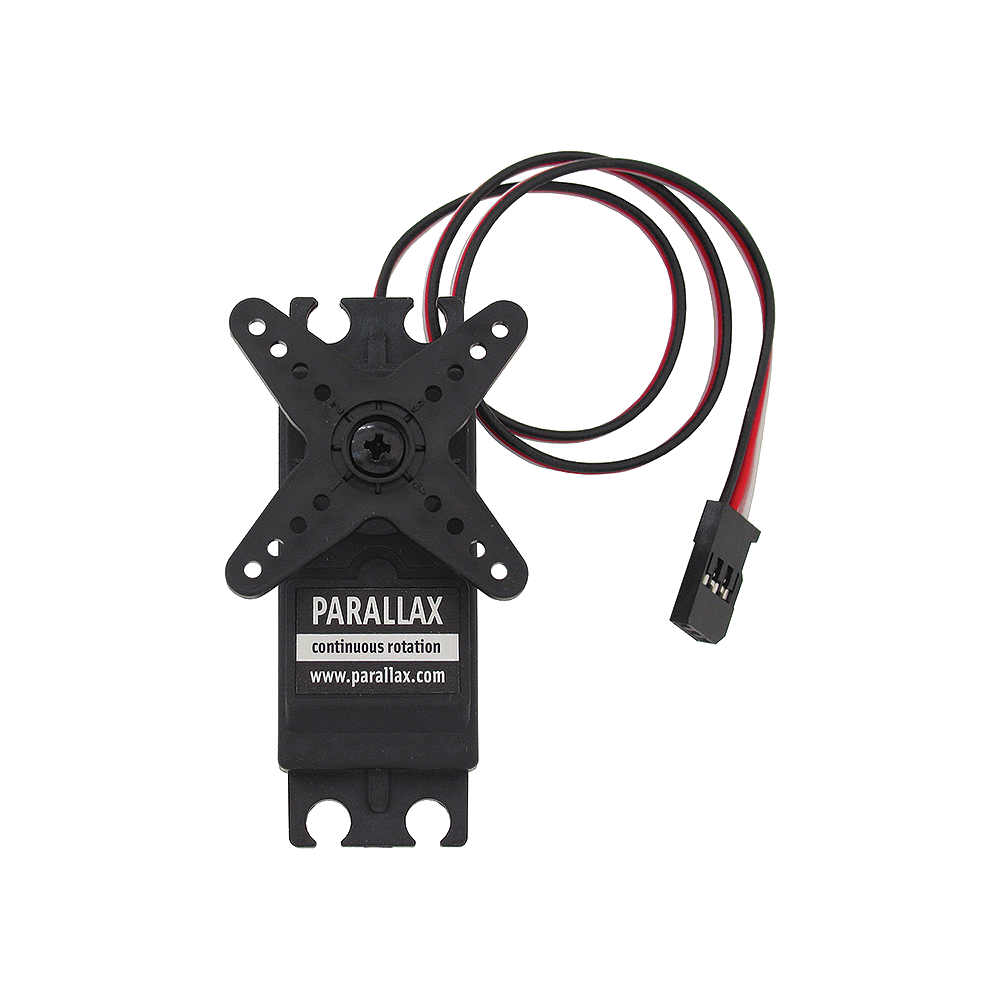
\includegraphics[scale = 0.2]{servo.png}
		\caption{ Parallax continuous rotation servo motor}
		\label{fig:servo}
	\end{center}
\end{figure}

First thing you have to do with the servo is to calibration. For example, servo motor is supposed to stop when the servo pin is written 90. But, there might be cases where the motor might not be 100\% stopped when 90 is written to the servo pin. To calibrate, we have to write 90 to servo and rotate the small screw until the motor is completely stopped. We have two servo motors facing opposite sides. The list of servo pin values that need to written to each motor is given in \cref{tab:servo}

\begin{table}[tbh]
	\caption{Servo pin values to be written for each operation}
	\label{tab:servo}
	\begin{center}
		\begin{tabular}{|l|c|c|}
			\hline
			Operation 	& 	Left motor	&	Right motor \\ 	\hline 
			Forward 	& 	0 			&	190 		\\
			Backward 	& 	190			&	0 			\\ 
			Stop		&	90 			&	90 			\\
			Left rotate	&	0			&	0			\\
			Right rotate&	190			&	190			\\	\hline 
		\end{tabular}
	\end{center}
\end{table} 

Further, depending on the time period you write these values, we can determine the angle of rotation. If you left rotate for $200\;ms$ and $400 \;ms$, robot will turn 90 and 180 degrees respectively.\\

Below is snippet gives a basic idea on this.
\begin{verbatim}
// define servo pins as global variables
#define LEFT_servo = 9 
#define RIGHT_servo = 10

void setup() {
    // attach the servos to servo object
    leftServo.attach(LEFT_servo); 
    rightServo.attach(RIGHT_servo); 
}

void goRight() {
    leftServo.write(190);
    rightServo.write(190);
}

void goStop() {
    leftServo.write(90);
    rightServo.write(90);
}

void loop() {
    // rotate 90 degrees right
    goRight();
    delay(200);
    
    // stop
    goStop();
    
    // rotate 180 degrees right
    goRight();
    delay(200);
}
\end{verbatim}



% =================================================================================
\newpage
\section{Attacking Mechanism} \label{sec:attacking}
In this section, we explain details about the attacking mechanism installed in our robot. Our mechanism is a simpler flipper in front of the robot.

% =================================================================================
\newpage
\section{Display System}

% =================================================================================
\newpage
\section{Algorithm}

% =================================================================================
\newpage
\section{Sumo Bot Code}

% =================================================================================
\newpage
\section{LCD System Code}

% =================================================================================
\newpage
\section{List of Components}

% =================================================================================
\newpage
\section{Future Developments}


\end{document}